\documentclass[12pt,a4paper]{article}
\usepackage[utf8]{inputenc}
\usepackage{amsmath}
\usepackage{amsfonts}
\usepackage{amssymb}
\usepackage{graphicx}
\usepackage{fullpage}
\usepackage{alltt}
\usepackage{color}
\usepackage{natbib}
\usepackage{alltt}
\bibliographystyle{abbrvnat}
%\usepackage[margin=1.5cm]{geometry}
\author{Simo Tukiainen}

\newcommand*{\Nset}{\mathbb{N}}  % reaalilukujen joukko
\newcommand*{\Rset}{\mathbb{R}}  % reaalilukujen joukko
\newcommand*{\norm}[1]{\left\lVert#1\right\rVert}
\DeclareMathOperator{\cov}{cov}
\newcommand{\mat}[1]{\mathbf{#1}}
\newcommand{\thicktilde}[1]{\mathbf{\tilde{\text{$#1$}}}}

\DeclareRobustCommand*{\vec}[1]{\ensuremath{
\mathchoice{\mbox{\boldmath$\displaystyle#1$}}
           {\mbox{\boldmath$\textstyle#1$}}
           {\mbox{\boldmath$\scriptstyle#1$}}
           {\mbox{\boldmath$\scriptscriptstyle#1$}}}}
\def\testbx{bx}


\begin{document}



\noindent Programming exercise in computational physics \\
%\noindent \textbf{Final project} \\
\noindent Simo Tukiainen, 014007316 \\

\begin{center}
\LARGE
\textbf{Retrieval of atmospheric profiles using dimension reduction}
\end{center}

\section{Introduction}

Measurement of the Earth's atmosphere are crucial for 
monitoring and understanding the current state and possible 
time evolution of the atmosphere. Stratospheric ozone and
greenhouse gases such as CO$_2$ and CH$_4$ are examples
of the important constituents that require continuous 
global monitoring.

Often the data are collected using remote sensing instruments when
interesting parameters like number densities are retrieved from the 
measured spectrum using a model that contains all the relevant physics.
To retrieve key parameters from the data, an inverse problem
must be solved. Typically, the inverse problem is ill-posed meaning that
there are more unknown parameters than actual information in the data.
Often the problem is non-linear too, at least in atmospheric remote sensing 
applications, and iterative solving methods are needed.

In this work I demonstrate a) how to simulate ground-based direct Sun 
measurements at short-wave infrared wavelengths and b) how to retrieve 
vertical information about the atmosphere from the (simulated) 
measurements using the dimension reduction method. The method is 
presented in a general form, so that it can easily be adapted for other
applications. The simulator and the retrieval method are 
implemented using Fortran. All implementations are original code by the author.
This study was done in 2015 for the course
``Programming exercise in computational physics'' at University of Helsinki.


\section{Atmospheric transmission}

%Given the forward model $f(\vec{x})$,
%observations $\vec{y}=y_1,y_2,...,y_m$ and the state vector $\vec{x}=x_1,x_2,...,x_n$,
%the linearized forward model in some reference state $\vec{x}_r$ can be written
%\begin{equation}
%\vec{y}-f(\vec{x}_r)=\frac{\partial f(\vec{x})}{\partial \vec{x}}(\vec{x}-\vec{x}_r)+\vec{\epsilon}=\mat{K}(\vec{x}-\vec{x}_r)+\vec{\epsilon},
%\end{equation}
%where $\vec{\epsilon}$ is the measurement error and $\mat{K}$ is the $m \times n$ weighting function
%matrix also called the Jacobian which has the elements $K_{ij}=\partial f_i(\vec{x})/\partial x_j$.
%With the direct Sun geometry, the derivatives (in one point) can be easily
%computed analytically.
The solar radiation entering the atmosphere experiences absorption and scattering 
from the molecules and particles in the atmosphere. In this work I consider an instrument
that directly looks at the Sun and records spectrum at short-wave infrared (SWIR) wavelengths 
at around 1.6~$\mu m$. The scattering is negligible at these wavelengths 
and I will only deal with absorption from now on.

The absorption from the atmospheric molecules follows the famous Beer-Lambert law.
Assuming a discretized atmosphere with $n$ layers, and
only one absorbing gas for simplicity, the transmittance in one wavelength is
\begin{equation}
\tau=\exp\Big(-\sum_{i=1}^n\sigma_{i} x_{i} l_i\Big),
\end{equation}
where $\sigma_{i}$ is the absorption coefficient, or cross section, of the layer $i$, and $x_{i}$ and $l_i$ are the
corresponding number density and slant length of the layer.
In matrix notation for the whole spectral window with $m$ points I have the cross section 
matrix $\mat{S} \in \Rset^{m \times n}$, densities $\vec{x} \in \Rset^n$, and slant 
lengths $\vec{l} \in \Rset^n$. Now the slant densities are
\begin{equation}
  \vec{\bar{x}} = \vec{l}\circ\vec{x},
  \label{eq:slant_dens}
\end{equation}
where $\circ$ is the point-wise product, and the transmittance
\begin{equation}
  \vec{\tau} = \exp(-\mat{S}\vec{\bar{x}}),
\end{equation}
which has the Jacobian
\begin{equation}
  \label{full_jacobian}
  \mat{K}=\frac{\partial \vec{\tau}}{\partial \vec{\bar{x}}}=-\text{diag}(\vec{\tau})\mat{S},
\end{equation}
where $\mat{K} \in \Rset^{m \times n}$. 
At the SWIR wavelengths, the absorption cross-section is a function of pressure and temperature.
The fundamental theory behind the absorption line formation and the line
shape are covered in numerous textbooks such as \citet{Goody95,Liou02}.
The actual cross section calculation is not relevant for this study and I will
take the cross sections as input data. It should be only noted that
the retrieval of the vertical information is based on the temperature and
altitude dependence, thus \textit{altitude dependence}, of the line shape.

%However, in the dimension reduction
%retrieval, we estimate $\alpha$-parameters instead of
%gas densities of the individual layers.
%Using the log-normal distribution, the projection
%matrix $\mat{P}_k$ in Eq.~(\ref{log_normal_dist}) gives the
%mapping back to the full space
%\begin{equation}
%  \vec{x}_k=\exp(\mat{P}_k\vec{\alpha})\circ\vec{x}_0,
%  \label{eq:fullmap}
%\end{equation}
%and the Jacobian becomes
%\begin{equation}
%  \mat{K}_k=\frac{\partial\vec{\tau}}{\partial\vec{\alpha}}=\mat{K}\text{diag}(\vec{l}\circ\vec{x}_k)\mat{P}_k
%  \label{eq:dimred_jac}
%\end{equation}
%being $\mat{K}_k \in \Rset^{m \times h}$. 

\section{Profile retrieval}

The ground-based and Sun looking instrument measures solar light modified by the whole 
atmospheric column of myriad trace gases. Our retrieval problem is then to estimate vertical
information from the single spectrum. 
%The information
%comes from the pressure and temperature dependence of the Voigt line shape: absorption
%lines are wider close to the Earth (in high pressure) than higher up in the atmosphere.
Given the measured spectrum $\vec{y} \in \Rset^m$, where $m$ is the number of wavelengths,
I wish to approximate the state vector $\vec{x} \in \Rset^n$, where $n$ is the number of
atmospheric layers. The state vector $\vec{x}$ represents the densities of the
discretized forward model atmosphere, so that
\begin{equation}
  \hat{\vec{x}}=\mat{R}(\vec{y},\mat{C}_y),
\end{equation}
where $\hat{\vec{x}} \in \Rset^n$ is the retrieved state, $\mat{R}$ is the
\textit{retrieval method}, and $\mat{C}_y \in \Rset^{m \times m}$ the measurement
error covariance. However the measured, or in this case simulated, SWIR spectrum does not contain 
enough information to resolve all $\sim$50 altitude levels in any
meaningful way (the inverse problem is said to be \textit{ill-posed}). A commonly used solution
is to regulate, or constrain, the problem using a priori information about the
state vector $\vec{x}$, and use Bayes' theorem to combine information from the
prior and measurement in the estimation process
\begin{equation}
  \vec{\pi}(\vec{x}|\vec{y}) \propto \vec{\pi}(\vec{y}|\vec{x})\vec{\pi}(\vec{x}),
\end{equation}
where $\vec{\pi}(\vec{x}|\vec{y})$ is called the posterior, $\vec{\pi}(\vec{y}|\vec{x})$ is
the likelihood term, and $\vec{\pi}(\vec{x})$ the prior term. In the CH$_4$ profile retrieval the
prior is, in practice, our ``best guess'' profile $\vec{x}_0 \in \Rset^n$ having the error
covariance $\mat{C}_x \in \Rset^{n \times n}$. Assuming that the prior and error distributions
are independent Gaussian distributions and that the error has no bias component,
the posterior density can be written in another form
\begin{align}
  \label{eq:Gmodel}
  \vec{\pi}(\vec{x}|\vec{y}) \propto \exp\left(-\frac{1}{2}\left(\norm{\vec{y}-f(\vec{x})}_{\mat{C}_y}^2 + \norm{\vec{x}-\vec{x}_0}_{\mat{C}_x}^2\right)\right),
\end{align}
where $f \colon \Rset^n \to \Rset^m$ is the forward model. For linear models $f$, Eq.~(\ref{eq:Gmodel})
would lead to a Gaussian distribution, but in practice
the forward model $f$ is usually non-linear, at least in atmospheric remote sensing problems.
This means that the posterior distribution is non-Gaussian and the optimization problem
of Eq.~(\ref{eq:Gmodel}) must be solved in iterative way.

The prior term $\norm{\vec{x}-\vec{x}_0}_{\mat{C}_x}^2$ is a widely used way to regulate the retrieval process.
The solution is a smooth profile even though both $\vec{x}$ and $\vec{x}_0$ are defined in full state space.
However, the solution depends significantly on $\vec{x}_0$ and the relationship between
$\mat{C}_y$ and $\mat{C}_x$. Too loose prior distribution will easily lead to unstable solution, and too
tight will skew the result if $\vec{x}_0$ is far from the truth. Hence, the prior is usually
set relatively tight to substantially regulate the solution and to avoid any superfluous oscillation of the posterior.
%Finally, we note that the posterior of Eq.~(\ref{eq:Gmodel}) requires us to solve $n$ unknown parameters,
%typically of the order of 50--70. MCMC is not very useful for sampling
%such a high dimensional space, thus in atmospheric remote sensing problems Eq.~(\ref{eq:Gmodel}) is practically
%always solved by exploiting the gradient of the forward model.

\subsection{Dimension reduction method}
 
The dimension reduction method that I use in this work is based on the decomposition of the
prior covariance \citep[see e.g][]{MarzoukNajm,CuiEtAl}. The prior covariance
is first defined in the full state space, i.e. the covariance is a $n \times n $ matrix where $n$ is the
number of layers in the model atmosphere. The idea is to truncate the prior covariance so that
plausible profile candidates can be drawn from the reduced prior distribution with just a few parameters.
Consider a Gaussian prior
$\mat{X} \sim \mathcal{N}(\vec{x}_0,\mat{C})$, where $\vec{x}_0$ is the prior mean and
$\mat{C} \in \Rset^{n \times n}$ is a positive-definite covariance matrix.
The covariance $\mat{C}$ can be factorized with
\begin{equation}
  \mat{C} = \mat{U}\mat{\Lambda}\mat{U}^T=\sum_{i=1}^n \lambda_i \vec{u}_i \vec{u}_i^T,
\end{equation}
\begin{equation}
  \mat{U} = [\vec{u}_1,\dots,\vec{u}_n],\quad \mat{\Lambda} = \text{diag}(\lambda_1,\dots,\lambda_n),
\end{equation}
where $\vec{u}_1,\dots, \vec{u}_n$ are column vectors,
and $\lambda_1 \geq \lambda_2 \geq \cdots \geq \lambda_n > 0$
are the singular values (or equivalently the eigenvalues) of $\mat{C}$. I can now define
the \textit{reduction mapping} of
order $k$, $1\leq k < n$, $\mat{P}_k = [\sqrt{\lambda_1}\vec{u}_1,\dots,\sqrt{\lambda_k}\vec{u}_k]$, and then consider the matrix truncation of order $k$
\begin{align}
  \thicktilde{\mat{C}} = \mat{P}_k \mat{P}_k^T = \sum_{i=1}^k \lambda_i\vec{u}_i\vec{u}_i^T,
  \label{eq:pmat}
\end{align}
where $\mat{P}_k \in \Rset^{n \times k}$ is the so-called projection matrix, and
$\thicktilde{\mat{C}} \in \Rset^{n \times n}$ approximates the original covariance.
This allows as to parametrize the new profile with $k$ parameters
\begin{equation}
  \label{gaussian_dist}
  \thicktilde{\vec{x}} = \vec{x}_0 + \mat{P}_k\vec{\alpha},
\end{equation}
where $\vec{\alpha} \in \Rset^{k}$ and furthermore $\vec{\alpha} \sim \mathcal{N}(0,\mat{I}_k)$.
The expectation value
\begin{equation}
\mathbb{E}(\thicktilde{\vec{x}})=\vec{x}_0 + \mathbb{E}(\mat{P}_k\vec{\alpha})=\vec{x}_0 + \mat{P}_k\mathbb{E}(\vec{\alpha})=\vec{x}_0,
\end{equation}
and the covariance
\begin{equation}
\cov(\thicktilde{\vec{x}})=\cov(\mat{P}_k\vec{\alpha})=\mat{P}_k\cov(\vec{\alpha})\mat{P}_k^T=\thicktilde{\mat{C}}.
\end{equation}
Hence, the profiles drawn using the reduced covariance approximate
the original distribution accurately if the neglected singular values are small.
%In addition to the Gaussian distribution used in Eq.~(\ref{gaussian_dist}), I can use the
%log-normal prior distribution
%\begin{equation}
%  \label{log_normal_dist}
%  \tilde{\vec{x}} = \exp(\mat{P}_k\vec{\alpha})\vec{x}_0,
%\end{equation}
%which always leads to positive profiles, assuming $\vec{x}_0$ is positive. 
Furthermore, the Jacobian in Eq.~(\ref{full_jacobian})
is straightforward to transform for the parametrized profile
\begin{equation}
  \mat{K}_k=\frac{\partial\vec{\tau}}{\partial\vec{\alpha}}=\mat{K}\text{diag}(\vec{l})\mat{P}_k
  \label{eq:dimred_jac}
\end{equation}
being $\mat{K}_k \in \Rset^{m \times k}$.

In the dimension reduction based profile retrieval, I try to find $\alpha$ parameters
that minimize the cost function. It is easy to see that the posterior distribution now becomes
\begin{align}
  \label{our_post}
  \vec{\pi}(\vec{\alpha}|\vec{y}) \propto \exp\left(-\frac{1}{2}\left(\norm{\vec{y}-f(\tilde{\vec{x}})}_{\mat{C}_y}^2 + \norm{\vec{\alpha}}_{\mat{I}_k}^2\right)\right),
\end{align}
where $\vec{y} \in \Rset^m $ is the measurement,
$f \colon \Rset^n \to \Rset^m$ is the forward model, and
$\mat{C}_y \in \Rset^{m \times m}$ is the measurement error covariance.
$\mat{I}_k \in \Rset^{k \times k}$ is the prior covariance of the $\alpha$ parameters i.e.
a diagonal unit matrix.
In practice, the relative contribution of the prior term in Eq.~(\ref{our_post}) is quite small.
Typically there are many more wavelengths in the spectral fitting
than $\alpha$ parameters, and the state vector (profile shape) has a significant
impact on the residuals. Thus, in most cases the likelihood term $\norm{\vec{y}-f(\tilde{\vec{x}})}_{\mat{C}_y}^2$ dominates the cost function.
While Eq.~(\ref{eq:Gmodel}) and Eq.~(\ref{our_post}) are analogous, the difference
is that in the dimension reduction retrieval the likelihood term
receives only smooth realization of $\tilde{\vec{x}}$ but in Eq.~(\ref{eq:Gmodel}) the state
vector $\vec{x}$ has no such restriction.

\section{Optimization}

One of the key benefits of the dimension reduction is that the number of estimated
parameters diminishes drastically (e.g. from 50 to 3). Thus, it would be feasible, 
and highly recommended, to statistically sample the full posterior distribution 
using the Markov chain Monte Carlo method (MCMC). However, this would be out of the scope
of this work and I use derivative-based optimization instead.

\subsection{Levenberg-Marquardt method}
\label{LM}

For the optimization of the $\alpha$ parameters in Eq.~(\ref{our_post}) I use the 
the Levenberg-Marquardt method. 
It is a derivative based, iterative optimization algorithm commonly used
for the nonlinear least squares problems, initially proposed by \citet{Levenberg44}. The iteration is defined
\begin{equation}
\vec{x}_{i+1} = \vec{x}_i + (\mat{K}^T\mat{K}+\gamma_i \text{diag}(\mat{K}^T\mat{K}))^{-1}\mat{K}^TR(\vec{x}_i)
\end{equation}
where $\mat{K}$ is the Jacobian and $R(\vec{x}_i)$ is the residual function.
In the original version of the method, the parameter $\gamma_i$ was chosen in each iteration to minimize
the cost function. This increases the computational burden and \citet{Marquardt63} proposed to find such $\gamma_i$
that simply reduces the cost function, no matter how much. The value of $\gamma_i$ is usually scaled (multiplied or divided) by
the factor of ten, until the cost function decreases, but the choice depends on the application.
Commonly, LM algorithms are chosen to stop with respect to some norms e.g. if 
the difference in residuals $\norm{R(\vec{x}_{i+1})-R(\vec{x_i})}$ is small.

\section{Implementation}

I have implemented all algorithms using Fortran (2003 standard). The code contains
five modules in separate files and one main program for testing (Fig.~1).
\begin{figure}[h!]
  \label{fig:vuo}
  \centering
  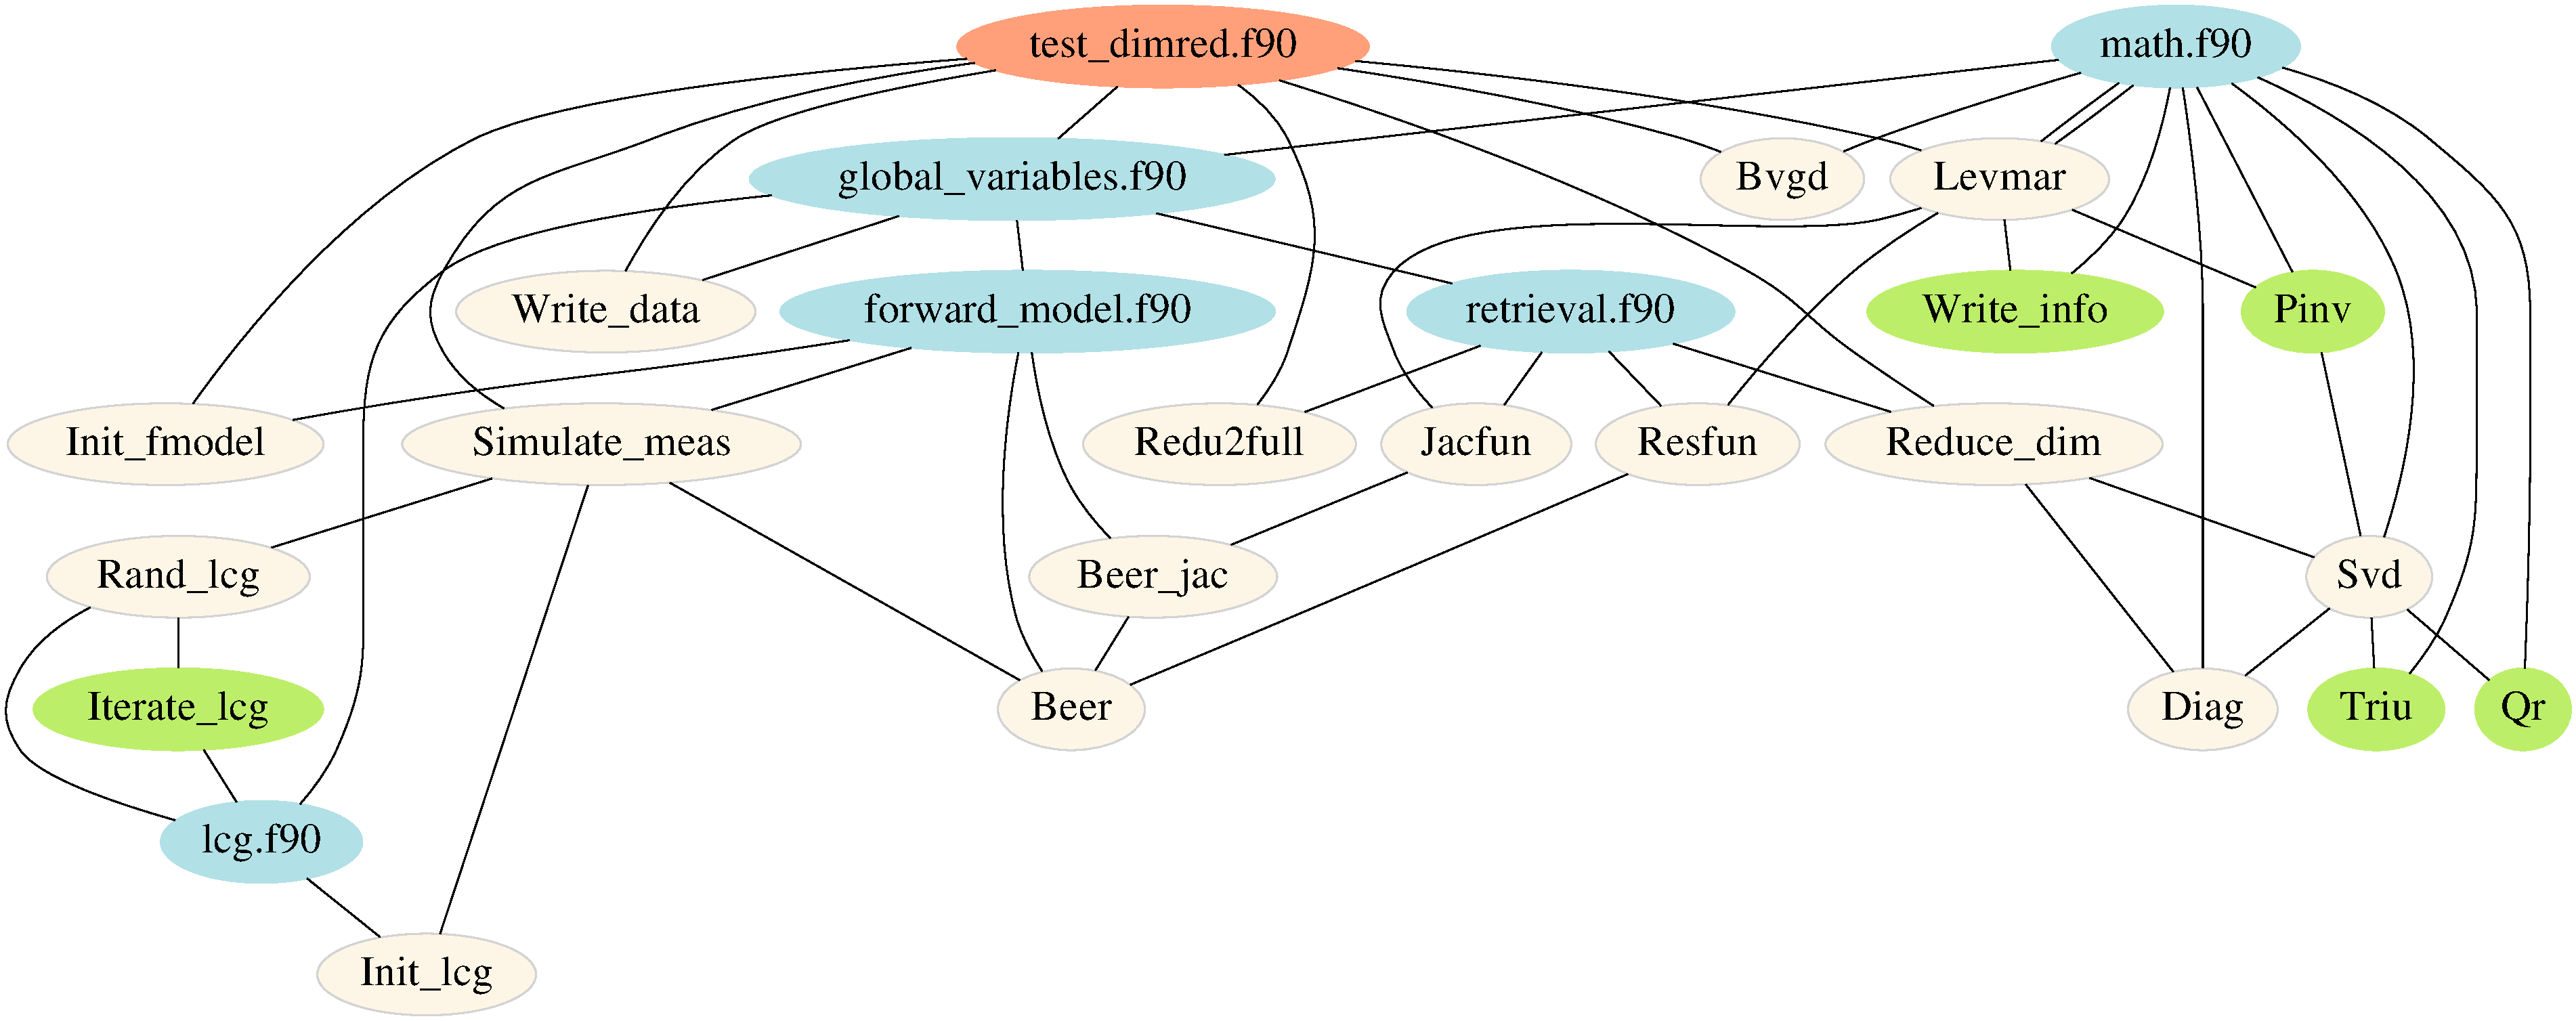
\includegraphics[width=1.05\textwidth]{figs/dimred_full.pdf}
  \caption{Modules (blue), public functions (light), private functions (green), main program (red), and their connections.}  
\end{figure}

The implementation is only for educational purposes so the physics contain a few simplifications:
\begin{itemize}
  \item Path lengths inside the atmospheric layers are not calculated nor taken account. I assume that all layers are 1~km thick (and the instrument points straight to the zenith). 
  \item There is only one trace gas (CH$_4$) and neutral air density in the atmosphere.
  \item I have an ideal instrument, thus the instrument function is not taken account.
\end{itemize}
The simulated spectrum is shown in Fig.~2. I have used a narrow bandwidth that contains five CH$_4$ absorption lines.
\begin{figure}[h]
  \label{fig:simuspec}
  \centering
  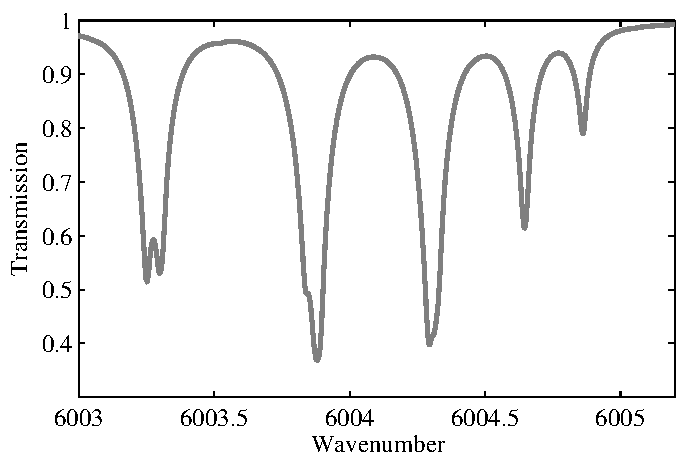
\includegraphics[width=0.5\textwidth]{figs/simu_spectrum.pdf}
  \caption{Simulated measurement.}
\end{figure}


The prior covariance is defined using two bivariate Gaussian distribution centered at 25~km (large variation) and 5~km (small variation).
This is sufficient for the simulation experiment but with real data the covariance should be approximated using accurate measurements, e.g. balloon observations, or model data.
The prior covariance is shown in Fig.~3.
\begin{figure}[h]
  \centering
  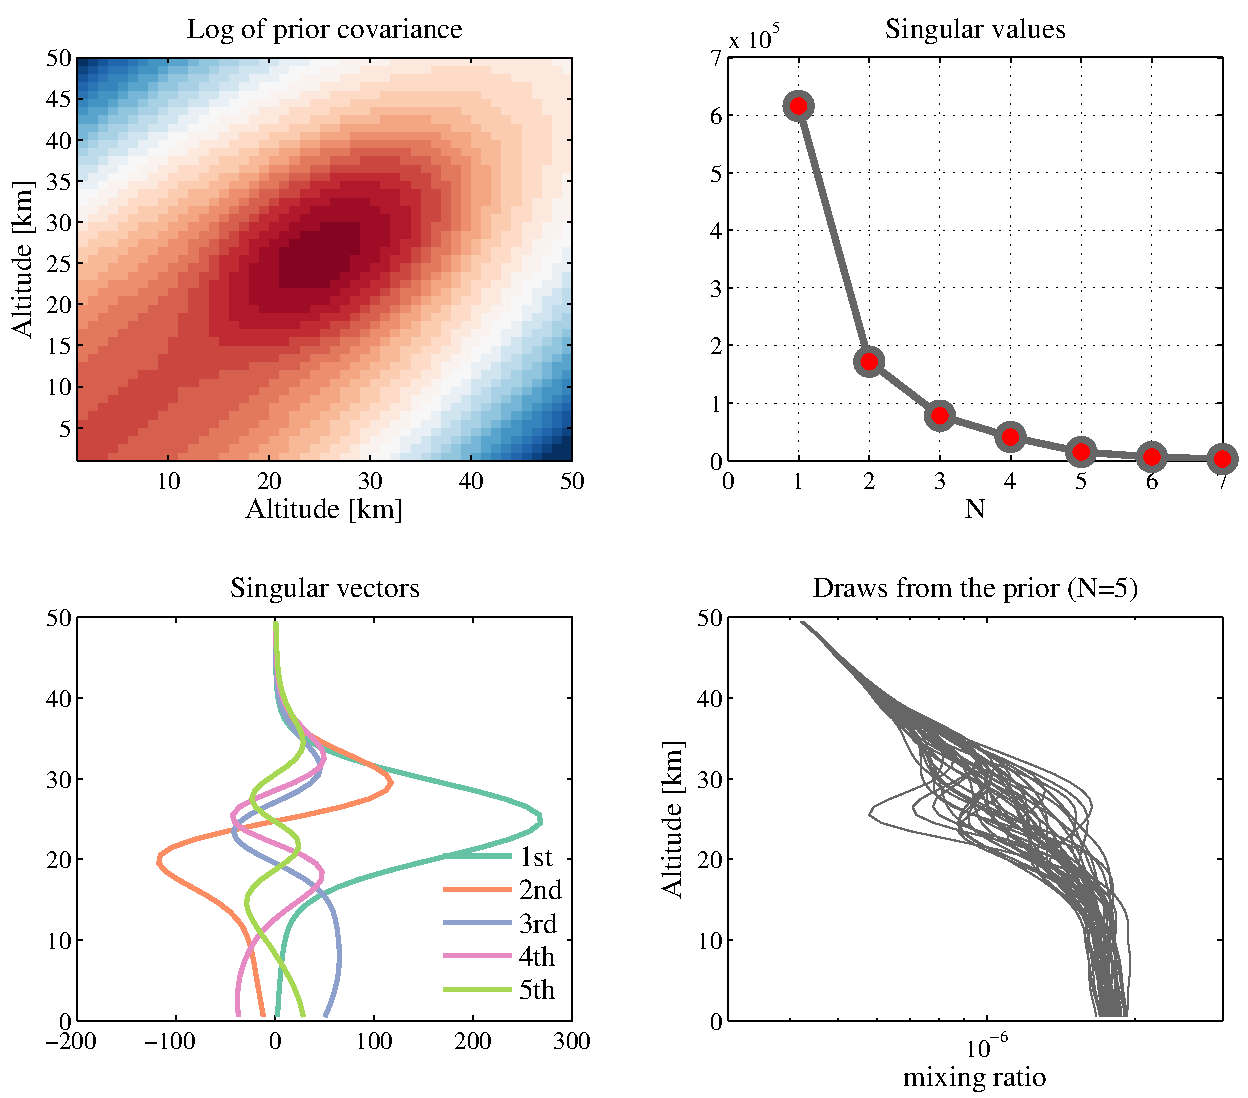
\includegraphics[width=0.8\textwidth]{figs/special_covariance.pdf}  
  \caption{Logarithm of the CH$_4$ prior covariance (upper-left), seven largest singular values (upper-right),
    five largest singular vectors (lower-left),
    and random draws from the prior using the five singular vectors (lower-right).}
  \label{cov}
\end{figure}


\subsection{Key algorithms}

In this section I present in more detail the implementation of the algorithms needed in this work.

\subsubsection{QR decomposition}
\begin{itemize}
  \setlength\itemsep{0.1cm}
 \item \textbf{name of the routine:} Qr
 \item \textbf{in file:} math.f90
 \item \textbf{used by:} Svd
\end{itemize}
%The QR algorithm is one of the most important algorithms in eigenvalue computations. 
The QR decomposition is the key procedure used in this work, and a 
fundamental matrix operation in general.
In the QR decomposition, the input matrix $\mat{A}$ is decomposed
into an orthogonal and triangular matrix:
\begin{equation}
\mat{A} =
\begin{bmatrix}
a_{11}   & a_{12}   & \cdots           & a_{1\mathrm{n}} \\
a_{21}   & a_{22}   & \cdots           & a_{2\mathrm{n}}\\
\vdots   & \vdots   & \ddots           & \vdots    \\
a_{\mathrm{m}1}     & a_{\mathrm{m}2} & \cdots  & a_{\mathrm{m}\mathrm{n}}  \\
\end{bmatrix}=
\begin{bmatrix}
q_{11}   & q_{12}   & \cdots           & q_{1\mathrm{m}} \\
q_{21}   & q_{22}   & \cdots           & q_{2\mathrm{m}}\\
\vdots   & \vdots   & \ddots           & \vdots    \\
a_{\mathrm{m}1}     & a_{\mathrm{m}2} & \cdots  & a_{\mathrm{m}\mathrm{m}}  \\
\end{bmatrix}
\begin{bmatrix}
r_{11}   & r_{12}   & \cdots           & r_{1\mathrm{n}} \\
0   & r_{22}   & \cdots           & r_{2\mathrm{n}}\\
\vdots   & \ddots   & \ddots           & \vdots    \\
0     & \cdots & 0  & r_{\mathrm{m}\mathrm{n}}  \\
\end{bmatrix}
\end{equation}
The QR decomposition is the basis of the iterative QR algorithm for finding eigenvalues, and
it can be used for finding singular values, too.
I have implemented the QR decomposition as the modified Gram-Schmidt (MGS) process \citep{Golub}. Applying MGS to
the column vectors of a full column rank matrix yields the QR decomposition.

\subsubsection{Singular value decomposition}
\begin{itemize}
 \item \textbf{name of the routine:} Svd
 \item \textbf{in file:} math.f90
 \item \textbf{used by:} Pinv, Reduce\_dim
\end{itemize}
SVD is the main algorithm in this work because it is used in the factorization of the prior
covariance. SVD is also needed in the pseudo-inverse function used by 
the Levenberg-Marquardt algorithm. 
Singular value decomposition is a factorization of a $m \times n$ matrix 
$\mathrm{\bf{A}}$ to the form
\begin{equation}
\mathrm{\bf{A}}=\mathrm{\bf{U}}\mathrm{\bf{S}}\mathrm{\bf{V}}^T,
\end{equation}
where $\mathrm{\bf{U}}$ is a $m \times m$ unitary matrix and
$\mathrm{\bf{V}}^T$ is a  $n \times n$ unitary matrix, so that
\begin{equation}
\mathrm{\bf{U}}^T\mathrm{\bf{U}}=\mathrm{\bf{I}}
\end{equation}
and
\begin{equation}
\mathrm{\bf{V}}^T\mathrm{\bf{V}}=\mathrm{\bf{I}}
\end{equation}
The matrix $\mathrm{\bf{S}}$ is a $m \times n$ rectangular diagonal matrix and its diagonal
values are called the singular values of $\mathrm{\bf{A}}$.
SVD is closely related to the eigenvalue decomposition of a symmetric matrix and the numerical
implementations of both decompositions
are similar, too. The general idea of all SVD algorithms is to find                                                                                                                                                
square roots of eigenvalues of $\mathrm{\bf{A}}^T$$\mathrm{\bf{A}}$ without actually
having to have to compute it.       

The concept of the SVD implementation in this work is to 
use the QR decomposition on $\mat{A}$  to iteratively ``pull'' $\mat{U}$ out from
the left and then use QR on  $\mat{A}^T$ to ``pull'' $\mat{V}$ out from the right.
This process makes $\mat{A}$ lower triangular and then upper triangular 
alternately, and eventually $\mat{A}$ becomes diagonal matrix with the singular 
values on the diagonal.

\subsubsection{Pseudo inverse}
\begin{itemize}
 \item \textbf{name of the routine:} Pinv
 \item \textbf{in file:} math.f90
 \item \textbf{used by:} Levmar
\end{itemize}
Pseudo inverse is the general inverse of a $m \times n$ matrix $\mat{A}$, where the
result is a $n \times m$ matrix $\mat{B}$ so that 
$\mat{ABA} = \mat{A}$, $\mat{BAB}$ = $\mat{B}$, and $\mat{AB}$ and $\mat{BA}$
are Hermitian. Pseudo inverse is convenient to implement using the SVD:
\begin{equation}
\mat{A}=\mat{U}\mat{S}\mat{V}^T
\end{equation} 
so it follows 
\begin{equation}
\mat{A}^{-1}=\mat{V}\mat{S}^{-1}\mat{U}^T,
\end{equation} 
where $\mat{S}^{-1}$ is trivial to calculate because $\mat{S}$ is a diagonal matrix.

\subsubsection{Levenberg-Marquardt}
\begin{itemize}
 \item \textbf{name of the routine:} Levmar
 \item \textbf{in file:} math.f90
 \item \textbf{used by:} test\_dimred (main program)
\end{itemize}
The idea of the Levenberg-Marquardt method is explained in Sect.~\ref{LM}. I have tried to implement the LM algorithm as generally as possible. 
It takes the residual and Jacobian functions and the data structure as input. The variable ``theta'' contains initial, and finally optimized, values
of the fitted parameters. The error covariance of the fitted parameters is estimated from the optimum with $(\mat{K}\mat{K}^T)^{-1}$, where
$\mat{K}$ is the Jacobian at the optimum.

\subsubsection{Bivariate Gaussian distribution}
\begin{itemize}
 \item \textbf{name of the routine:} Bvgd
 \item \textbf{in file:} math.f90
 \item \textbf{used by:} test\_dimred (main program)
\end{itemize}
The prior covariance is generated using two Gaussian bivariate distributions. 
%This might not be the most typical way to generate
%covariance matrices but 
A bivariate Gaussian distribution can be defined in 2-dimensional nonsingular case
\begin{equation}
f(x,y)=\frac{1}{2\pi\sigma_x\sigma_y\sqrt{1-\rho^2}}\exp\Bigg(-\frac{1}{2(1-\rho^2)}\bigg[\frac{(x-\mu_x)^2}{\sigma_x^2}+\frac{(y-\sigma_y^2)^2}{\sigma_y^2}-\frac{2\rho(x-\mu_x)(y-\mu_y)}{\sigma_x\sigma_y}\bigg]\Bigg),
\end{equation}
where $\mu_x$ and $\mu_y$ describe the mean point of the distribution, $\sigma_x$ and $\sigma_y$ are the deviations in $x$ and $y$ direction, and $\rho$ is the correlation length.

\subsubsection{Measurement noise}
\begin{itemize}
 \item \textbf{name of the routine:} Simulate\_meas
 \item \textbf{in file:} forward\_model.f90
 \item \textbf{used by:} test\_dimred (main program)
\end{itemize}
In this work the measurement noise model is additive, normally distributed noise. Random numbers 
can be drawn from the standard normal distribution using the simple method
\begin{equation}
r_n=\sum_{i=1}^N(r_i)-\frac{N}{2}
\end{equation}
where $r$ is an ordinary (pseudo) random number between 0-1. For $N\rightarrow \infty$, the 
distribution of the sum becomes Gaussian. This is a famous rule in statistics and the proof
is not relevant here.

\subsubsection{Random number generator}
\begin{itemize}
 \item \textbf{name of the routine:} Init\_lcg, Rand\_lcg
 \item \textbf{in file:} lcg.f90
  \item \textbf{used by:} Simulate\_meas
\end{itemize}
As a random number generator I use the the linear congruential generator. It is a simple
method for generating pseudo random numbers. The number are generated using the 
recurrence relation:
\begin{equation}
X_{n+1}=(aX_n+c) \mod m
\end{equation}
where $m, m>0$ is called the ``modulus'', $a, 0<a<m$ the ``multiplier'' and $c, 0\leq c<m$ the ``increment''.
The starting value $X_0, 0 \leq X_0 <m$ is called the ``seed''. Here $X_0=123123$ and the other parameters
are taken from \citet{PressEtAl92}: $m = 4294967296$, $a=1664525$, and $c=1013904223$.

\subsection{Input data}
The program needs following input data in order to simulate the measurement:
\begin{itemize}
\item atmosphere (file \textbf{atmos.dat}). It contains altitudes, ``true'' density profile that I use in the simulation of the measurement, prior profile, and neutral air density profile.
\item cross sections (file \textbf{abs\_coef.dat})
\end{itemize}

\subsection{Output}

Running the program will write information about simulation set-up and the retrieval results to several 
text files in the output/ folder. The output files are shown in Table~1. If the program is launched multiple 
times, the old files will be always overwritten.
\begin{table}[h!]
\begin{center}
\begin{tabular}{c | c | l}
file name & dimensions & description \\
\hline
d.dat & 1 & number of used principal components \\ 
alt.dat & nalt & altitude vector \\
dens.dat & nalt & ``true'' profile used in simulation \\
prior.dat & nalt & prior profile \\
air.dat & nalt & air density profile \\
profile.dat & nalt& retrieved profile \\
t.dat & nwl & simulated transmission \\
wl.dat & nwl & wl vector \\
r.dat & nwl+d & residual \\
C.dat &nalt$\times$nalt & prior covariance matrix \\
P.dat & nalt$\times$d & projection matrix\\
q.dat & nalt & singular values of C \\
\hline
\end{tabular}
\caption{Output files}
\end{center}
\end{table}
The results can be visualized with the Matlab function \textbf{plot\_dimred\_results.m} which is included in the root directory.

\subsection{Example run}

This is a example session how to obtain the code, compile, run, and visualize main results with Matlab. Red text is commentary.

\begin{alltt}
$ wget https://dl.dropboxusercontent.com/u/27553525/dim_red_retrieval.tar.gz
$ tar -xzvf dim_red_retrieval.tar.gz                \textcolor{red}{unpack}
$ cd dim_red_retrieval/                             \textcolor{red}{move to the root folder}
$ make                                              \textcolor{red}{compile all modules}
$ ./test_dimred                                     \textcolor{red}{run the program}

 Give std of noise. Signal is between 0-1 and the noise is additive ~ N(0,std^2)
 Common value is e.g. 0.001 but you can try different values..
0.0001                                              \textcolor{red}{set noise level..}
  Give number of principal components (~2-5 is good)  
5                                                   \textcolor{red}{give number of components..}
 ----------------------------------
 Iteration     RSS          lam
 ----------------------------------
     0    5632.5160474     1.0E-03
     1       2.2121584     1.0E-03
     2       1.1082433     1.0E-04
     3       1.0207569     1.0E-05
     4       1.0039673     1.0E-06
     5       1.0019448     1.0E-07
     6       1.0019454     1.0E-06

$ matlab -nodesktop                               \textcolor{red}{launch matlab}
$ plot_dimred_results                             \textcolor{red}{plot some results}
\end{alltt} 

\section{Results}

The shape of the proposal profiles depend on the covariance itself and the number of principal components 
that are used to approximate the original covariance. The available information content in the signal 
is limited by the measurement noise. Figure 4 shows example retrievals using different
number of principal components (from top row to down: 1, 2, 3, 5) and noise $\sigma=0.001$. The panels on the right
show the corresponding residuals. It can be easily seen from the residual where the information about the
vertical structure is coming. Furthermore, 1-2 principal components is not enough to find the true profile, but no more 
than 3 pieces of information can be retrieved due to the noise.
\begin{figure}[h]
  \label{simu_results}
  \centering
  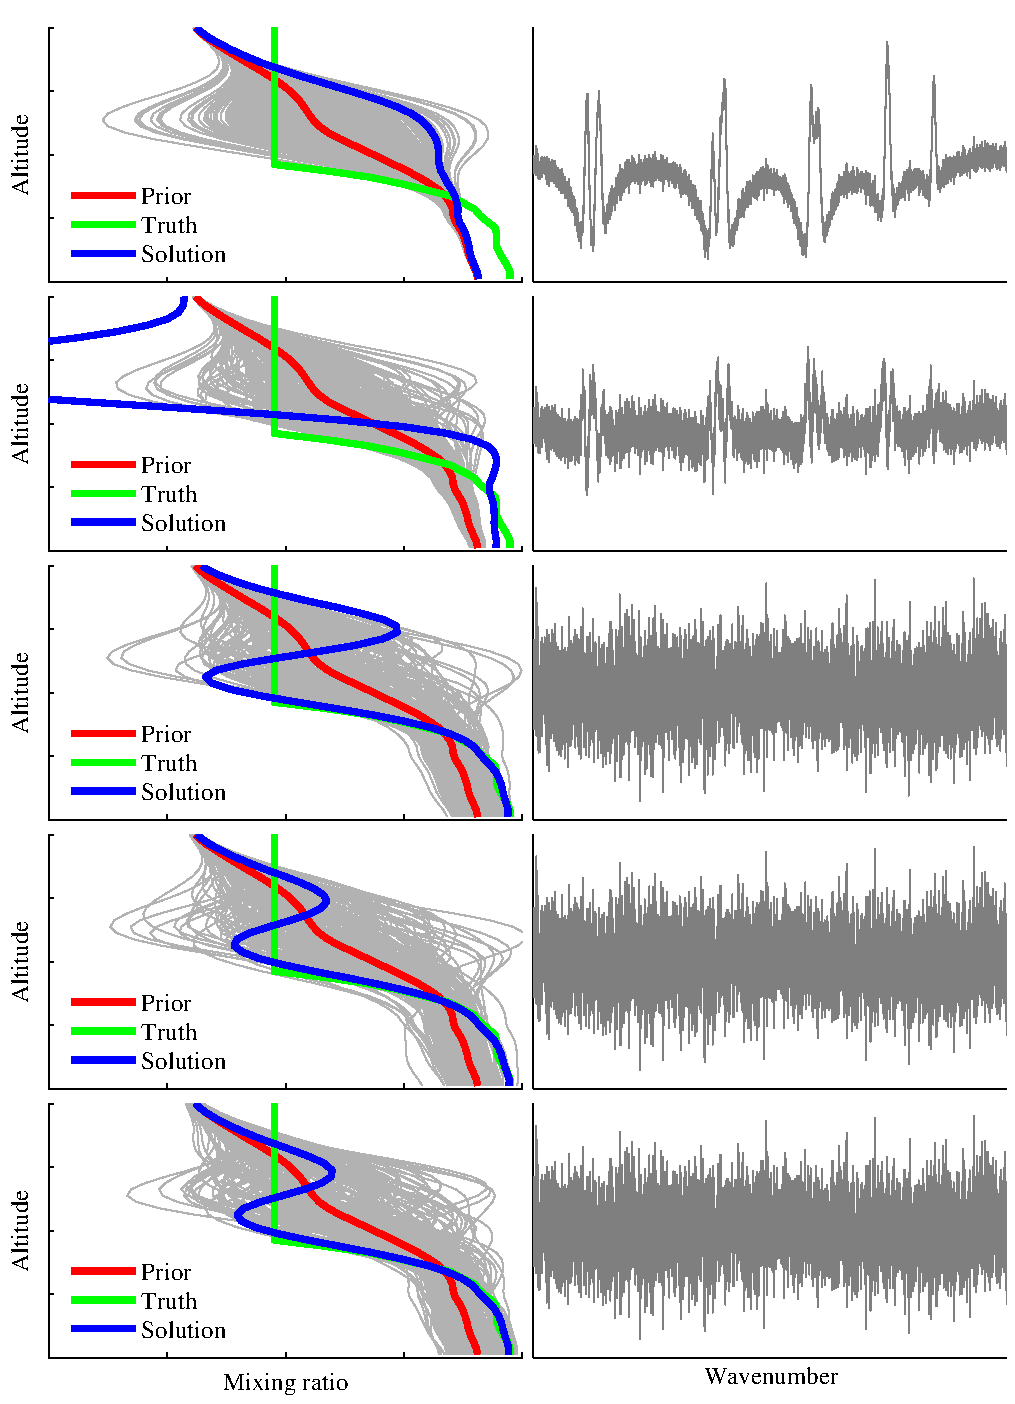
\includegraphics[width=0.9\textwidth]{figs/special_solution.pdf}
  \caption{Left panels: prior profile (red), solution (blue), truth (green) and random draws from the prior (grey). Right panels: corresponding residuals. Different rows 
    represent different number of principal components: 1 (uppermost), 2, 3, 4, and 5 (lowermost).}
\end{figure}

\section{Discussion}

In this study I implemented and tested a dimension reduction based retrieval method. This kind
of technique can be used to decrease the number of estimated parameters in ill-posed inverse problems.
For testing the method I generated a noisy transmission signal and created a prior covariance that
was decomposed using the SVD. How well the method can find the true atmosphere depends on the
covariance structure (and marginally on the prior profile itself), number of used principal 
components, and the measurement noise.

Because in this work the main motivation was the actual implementation of the used algorithms, 
I somewhat simplified the physics of the problem and did not perform very comprehensive 
analysis on the results. However, the minimization seem to work as it should and the retrieved
profiles looks reasonable.

\newpage
\clearpage

\bibliography{references}

\end{document}
